\documentclass[tikz]{standalone}
\begin{document}
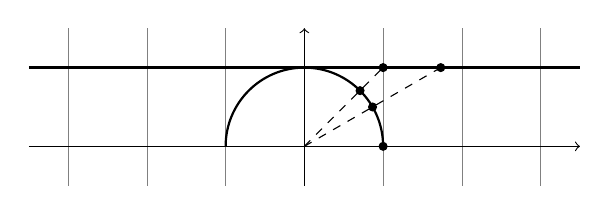
\begin{tikzpicture}
  \draw[help lines] (-3.5,-0.5) grid (3.5,1.5);
  \draw [->] (-3.5,0) -- (3.5,0);
  \draw [->] (0,-0.5) -- (0,1.5);
  \begin{scope}
    \clip (-3.5,0) rectangle (3.5,1.5);
    \draw[thick] (0,0) circle [radius=1];
  \end{scope}
  \draw[thick] (-3.5,1) -- (3.5,1);

  \draw[fill] (45:1cm) circle [radius=0.05];
  \draw[fill] (1,1) circle [radius=0.05];
  \draw[dashed] (0,0) -- (1,1);

  \draw[fill] (30:1cm) circle [radius=0.05];
  \draw[fill] (1.7320508075688774, 1) circle [radius=0.05];
  \draw[dashed] (0,0) -- (1.7320508075688774,1);

  \draw[fill] (0:1cm) circle [radius=0.05];
\end{tikzpicture}
\end{document}
